\documentclass[letterpaper,12pt]{article}
\usepackage[margin=.65in,top=.72in,bottom=.62in,headheight=16pt,headsep=15pt,footskip=19pt]{geometry}
\usepackage[T1]{fontenc}
\usepackage{lmodern,tikz,fancyhdr}\pdfmapfile{+lm.map}
\usetikzlibrary{arrows.meta,shapes.geometric}
\pagestyle{fancy}\fancyhf{}\renewcommand{\headrulewidth}{0pt}\renewcommand{\footrulewidth}{0pt}
\setlength{\parindent}{0pt}\setlength{\parskip}{0pt}
\fancyhead[L]{\small Week 43 / Shuffling picture cards / K--1}
\fancyfoot[L]{\footnotesize Bellingham Math Circle / Week 43 / W43-k-1-v2}\fancyfoot[R]{\footnotesize\thepage}
\begin{document}
\noindent\begin{tikzpicture}[x=1cm,y=1cm]\path[use as bounding box] (0,0) rectangle (18.2,-23.6);
\node[anchor=north west,text width=18cm,inner sep=0pt,font=\fontsize{14}{17}\selectfont] at (0,0) {\textbf{Problem 1:} Make every different row using these three cards once each.};
\draw[gray!65,rounded corners=2pt] (1.0,-1.7) rectangle (3.0,-3.9000000000000004);
\draw[fill=orange!22,line width=.8pt] (1.62,-3.026) rectangle (2.38,-2.266);
\node[anchor=north west,text width=1.8cm,inner sep=0pt,font=\fontsize{9}{12}\selectfont] at (1.15,-3.284) {A};
\draw[gray!65,rounded corners=2pt] (3.0,-1.7) rectangle (5.0,-3.9000000000000004);
\draw[fill=green!22,line width=.8pt] (4.0,-2.646) circle (0.38);
\node[anchor=north west,text width=1.8cm,inner sep=0pt,font=\fontsize{9}{12}\selectfont] at (3.15,-3.284) {B};
\draw[gray!65,rounded corners=2pt] (5.0,-1.7) rectangle (7.0,-3.9000000000000004);
\draw[fill=violet!22,line width=.8pt] (6.0,-2.266) -- (6.38,-3.026) -- (5.62,-3.026) -- cycle;
\node[anchor=north west,text width=1.8cm,inner sep=0pt,font=\fontsize{9}{12}\selectfont] at (5.15,-3.284) {C};
\draw[gray!65,rounded corners=2pt] (2.0,-5) rectangle (6.7,-11.1);
\node[anchor=north west,text width=1cm,inner sep=0pt,font=\fontsize{11}{14}\selectfont] at (2.15,-5.12) {1};
\draw[gray!65,rounded corners=2pt] (6.7,-5) rectangle (11.4,-11.1);
\node[anchor=north west,text width=1cm,inner sep=0pt,font=\fontsize{11}{14}\selectfont] at (6.8500000000000005,-5.12) {2};
\draw[gray!65,rounded corners=2pt] (11.4,-5) rectangle (16.1,-11.1);
\node[anchor=north west,text width=1cm,inner sep=0pt,font=\fontsize{11}{14}\selectfont] at (11.55,-5.12) {3};
\draw[gray!65,rounded corners=2pt] (0.0,-13.0) rectangle (2.6,-15.5);
\draw[gray!65,rounded corners=2pt] (2.6,-13.0) rectangle (5.2,-15.5);
\draw[gray!65,rounded corners=2pt] (5.2,-13.0) rectangle (7.800000000000001,-15.5);
\draw[gray!65,rounded corners=2pt] (9.0,-13.0) rectangle (11.6,-15.5);
\draw[gray!65,rounded corners=2pt] (11.6,-13.0) rectangle (14.2,-15.5);
\draw[gray!65,rounded corners=2pt] (14.2,-13.0) rectangle (16.8,-15.5);
\draw[gray!65,rounded corners=2pt] (0.0,-16.3) rectangle (2.6,-18.8);
\draw[gray!65,rounded corners=2pt] (2.6,-16.3) rectangle (5.2,-18.8);
\draw[gray!65,rounded corners=2pt] (5.2,-16.3) rectangle (7.800000000000001,-18.8);
\draw[gray!65,rounded corners=2pt] (9.0,-16.3) rectangle (11.6,-18.8);
\draw[gray!65,rounded corners=2pt] (11.6,-16.3) rectangle (14.2,-18.8);
\draw[gray!65,rounded corners=2pt] (14.2,-16.3) rectangle (16.8,-18.8);
\draw[gray!65,rounded corners=2pt] (0.0,-19.6) rectangle (2.6,-22.1);
\draw[gray!65,rounded corners=2pt] (2.6,-19.6) rectangle (5.2,-22.1);
\draw[gray!65,rounded corners=2pt] (5.2,-19.6) rectangle (7.800000000000001,-22.1);
\draw[gray!65,rounded corners=2pt] (9.0,-19.6) rectangle (11.6,-22.1);
\draw[gray!65,rounded corners=2pt] (11.6,-19.6) rectangle (14.2,-22.1);
\draw[gray!65,rounded corners=2pt] (14.2,-19.6) rectangle (16.8,-22.1);
\end{tikzpicture}
\newpage
\noindent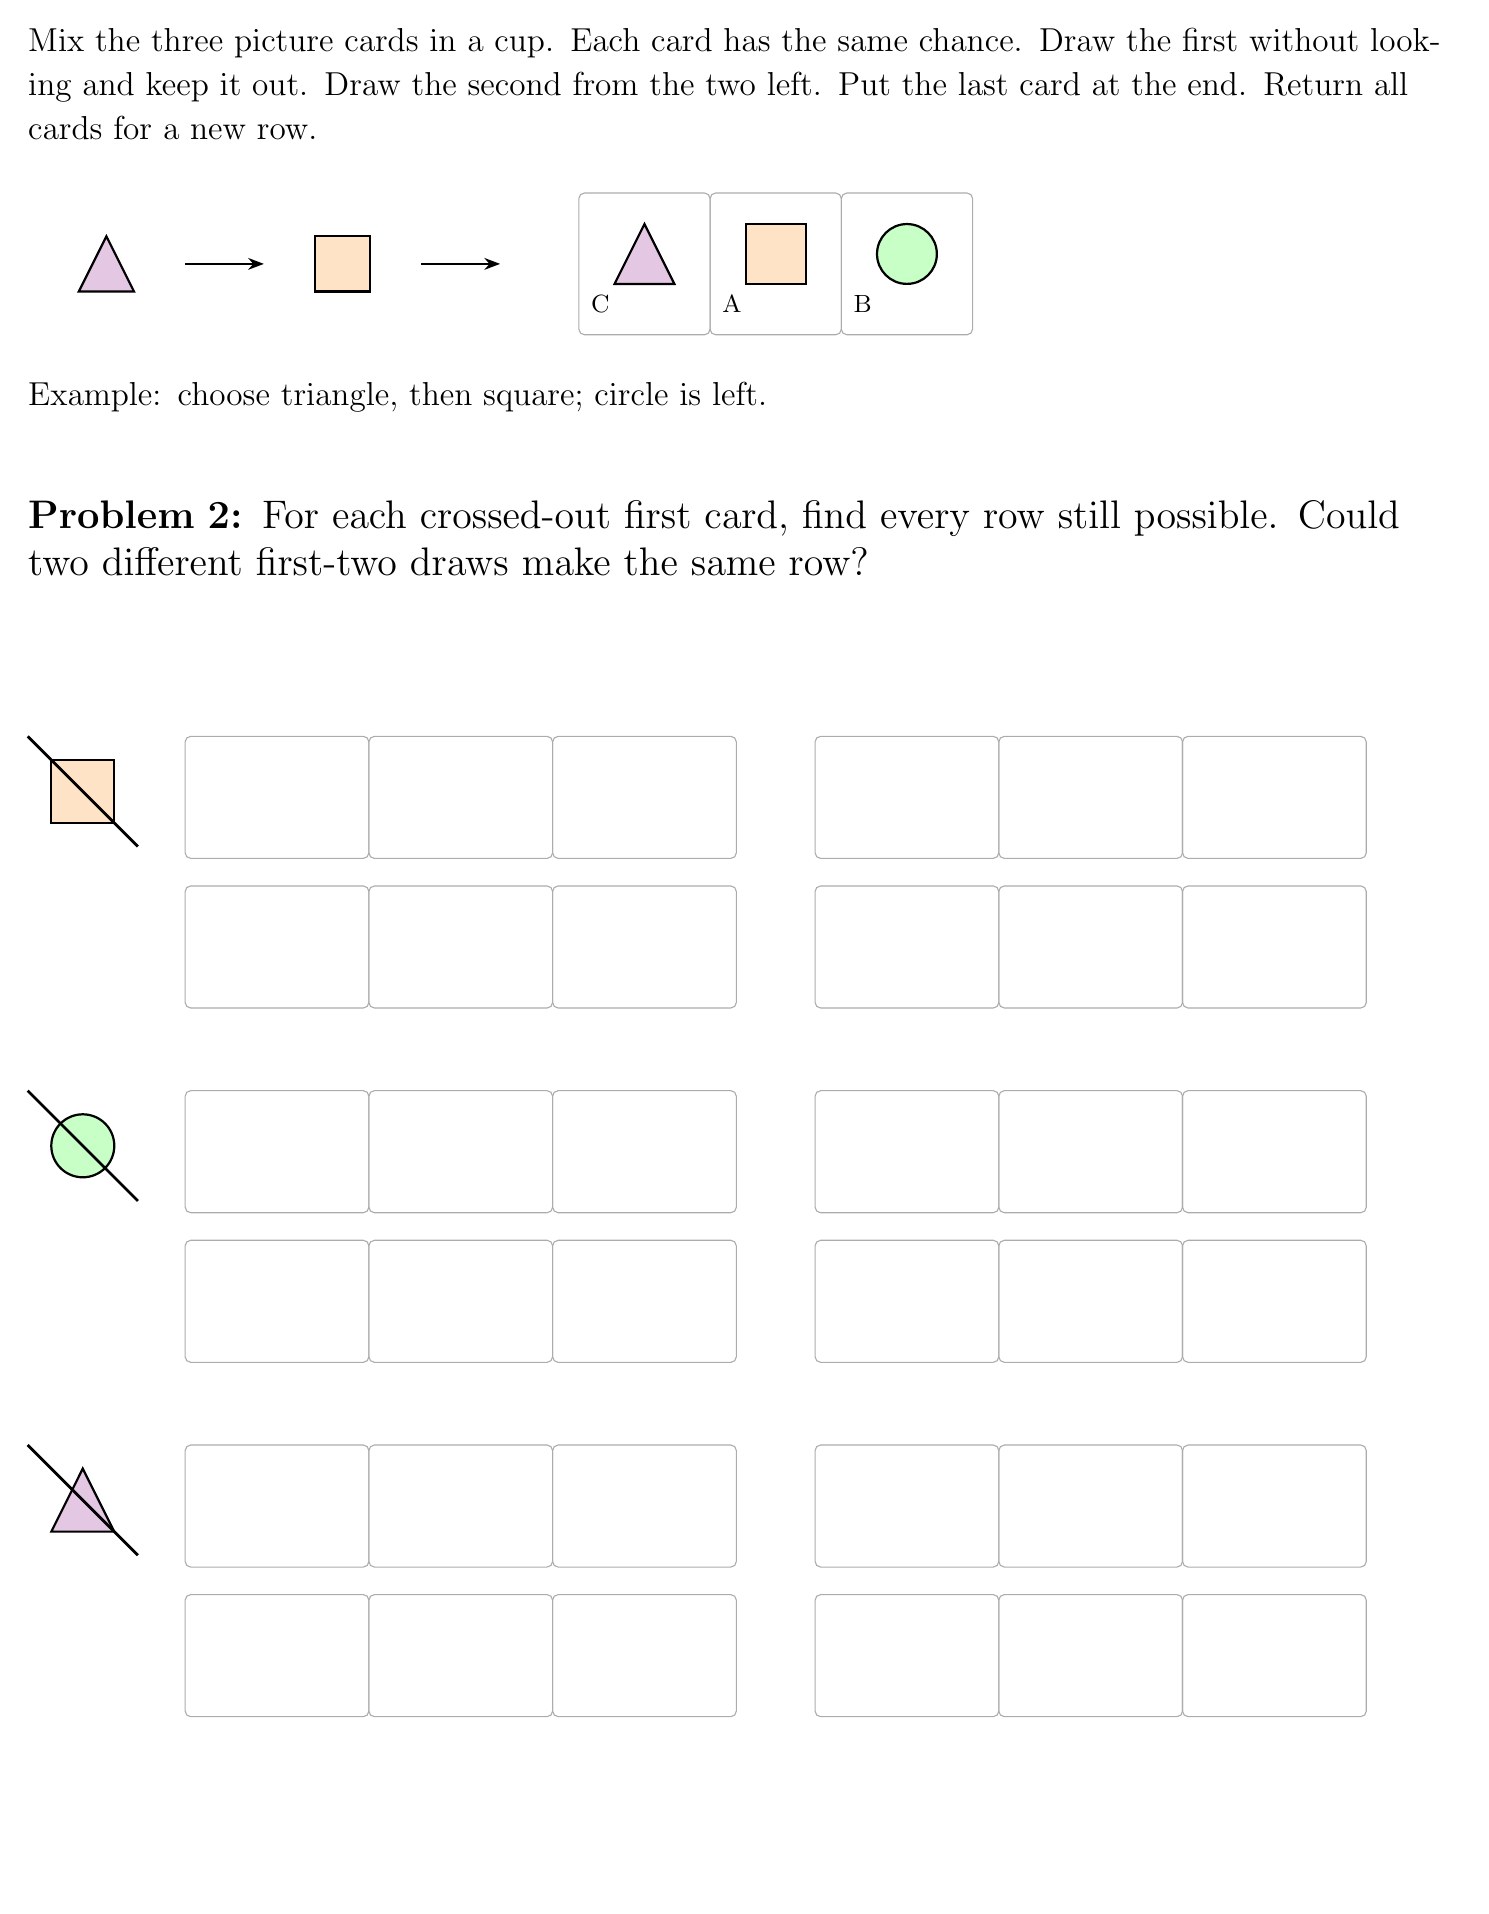
\begin{tikzpicture}[x=1cm,y=1cm]\path[use as bounding box] (0,0) rectangle (18.2,-23.6);
\node[anchor=north west,text width=18cm,inner sep=0pt,font=\fontsize{13}{16}\selectfont] at (0,0) {Mix the three picture cards in a cup. Each card has the same chance. Draw the first without looking and keep it out. Draw the second from the two left. Put the last card at the end. Return all cards for a new row.};
\draw[fill=violet!22,line width=.8pt] (1,-2.65) -- (1.35,-3.35) -- (0.65,-3.35) -- cycle;
\draw[-{Stealth[length=2mm]},line width=.8pt] (2,-3) -- (3,-3) node[midway,above,font=\small] {};
\draw[fill=orange!22,line width=.8pt] (3.65,-3.35) rectangle (4.35,-2.65);
\draw[-{Stealth[length=2mm]},line width=.8pt] (5,-3) -- (6,-3) node[midway,above,font=\small] {};
\draw[gray!65,rounded corners=2pt] (7.0,-2.1) rectangle (8.666666666666666,-3.9000000000000004);
\draw[fill=violet!22,line width=.8pt] (7.833333333333333,-2.494) -- (8.213333333333333,-3.254) -- (7.453333333333333,-3.254) -- cycle;
\node[anchor=north west,text width=1.4666666666666668cm,inner sep=0pt,font=\fontsize{9}{12}\selectfont] at (7.15,-3.396) {C};
\draw[gray!65,rounded corners=2pt] (8.666666666666666,-2.1) rectangle (10.333333333333332,-3.9000000000000004);
\draw[fill=orange!22,line width=.8pt] (9.12,-3.254) rectangle (9.88,-2.494);
\node[anchor=north west,text width=1.4666666666666668cm,inner sep=0pt,font=\fontsize{9}{12}\selectfont] at (8.816666666666666,-3.396) {A};
\draw[gray!65,rounded corners=2pt] (10.333333333333334,-2.1) rectangle (12.0,-3.9000000000000004);
\draw[fill=green!22,line width=.8pt] (11.166666666666668,-2.874) circle (0.38);
\node[anchor=north west,text width=1.4666666666666668cm,inner sep=0pt,font=\fontsize{9}{12}\selectfont] at (10.483333333333334,-3.396) {B};
\node[anchor=north west,text width=18cm,inner sep=0pt,font=\fontsize{12}{15}\selectfont] at (0,-4.5) {Example: choose triangle, then square; circle is left.};
\node[anchor=north west,text width=18cm,inner sep=0pt,font=\fontsize{14}{17}\selectfont] at (0,-6) {\textbf{Problem 2:} For each crossed-out first card, find every row still possible. Could two different first-two draws make the same row?};
\draw[fill=orange!22,line width=.8pt] (0.29999999999999993,-10.1) rectangle (1.1,-9.299999999999999);
\draw[line width=1pt] (0,-9.0) -- (1.4,-10.4);
\draw[gray!65,rounded corners=2pt] (2.0,-9.0) rectangle (4.333333333333334,-10.55);
\draw[gray!65,rounded corners=2pt] (4.333333333333334,-9.0) rectangle (6.666666666666668,-10.55);
\draw[gray!65,rounded corners=2pt] (6.666666666666667,-9.0) rectangle (9.0,-10.55);
\draw[gray!65,rounded corners=2pt] (10.0,-9.0) rectangle (12.333333333333334,-10.55);
\draw[gray!65,rounded corners=2pt] (12.333333333333334,-9.0) rectangle (14.666666666666668,-10.55);
\draw[gray!65,rounded corners=2pt] (14.666666666666668,-9.0) rectangle (17.0,-10.55);
\draw[gray!65,rounded corners=2pt] (2.0,-10.9) rectangle (4.333333333333334,-12.450000000000001);
\draw[gray!65,rounded corners=2pt] (4.333333333333334,-10.9) rectangle (6.666666666666668,-12.450000000000001);
\draw[gray!65,rounded corners=2pt] (6.666666666666667,-10.9) rectangle (9.0,-12.450000000000001);
\draw[gray!65,rounded corners=2pt] (10.0,-10.9) rectangle (12.333333333333334,-12.450000000000001);
\draw[gray!65,rounded corners=2pt] (12.333333333333334,-10.9) rectangle (14.666666666666668,-12.450000000000001);
\draw[gray!65,rounded corners=2pt] (14.666666666666668,-10.9) rectangle (17.0,-12.450000000000001);
\draw[fill=green!22,line width=.8pt] (0.7,-14.2) circle (0.4);
\draw[line width=1pt] (0,-13.5) -- (1.4,-14.9);
\draw[gray!65,rounded corners=2pt] (2.0,-13.5) rectangle (4.333333333333334,-15.05);
\draw[gray!65,rounded corners=2pt] (4.333333333333334,-13.5) rectangle (6.666666666666668,-15.05);
\draw[gray!65,rounded corners=2pt] (6.666666666666667,-13.5) rectangle (9.0,-15.05);
\draw[gray!65,rounded corners=2pt] (10.0,-13.5) rectangle (12.333333333333334,-15.05);
\draw[gray!65,rounded corners=2pt] (12.333333333333334,-13.5) rectangle (14.666666666666668,-15.05);
\draw[gray!65,rounded corners=2pt] (14.666666666666668,-13.5) rectangle (17.0,-15.05);
\draw[gray!65,rounded corners=2pt] (2.0,-15.4) rectangle (4.333333333333334,-16.95);
\draw[gray!65,rounded corners=2pt] (4.333333333333334,-15.4) rectangle (6.666666666666668,-16.95);
\draw[gray!65,rounded corners=2pt] (6.666666666666667,-15.4) rectangle (9.0,-16.95);
\draw[gray!65,rounded corners=2pt] (10.0,-15.4) rectangle (12.333333333333334,-16.95);
\draw[gray!65,rounded corners=2pt] (12.333333333333334,-15.4) rectangle (14.666666666666668,-16.95);
\draw[gray!65,rounded corners=2pt] (14.666666666666668,-15.4) rectangle (17.0,-16.95);
\draw[fill=violet!22,line width=.8pt] (0.7,-18.3) -- (1.1,-19.099999999999998) -- (0.29999999999999993,-19.099999999999998) -- cycle;
\draw[line width=1pt] (0,-18.0) -- (1.4,-19.4);
\draw[gray!65,rounded corners=2pt] (2.0,-18.0) rectangle (4.333333333333334,-19.55);
\draw[gray!65,rounded corners=2pt] (4.333333333333334,-18.0) rectangle (6.666666666666668,-19.55);
\draw[gray!65,rounded corners=2pt] (6.666666666666667,-18.0) rectangle (9.0,-19.55);
\draw[gray!65,rounded corners=2pt] (10.0,-18.0) rectangle (12.333333333333334,-19.55);
\draw[gray!65,rounded corners=2pt] (12.333333333333334,-18.0) rectangle (14.666666666666668,-19.55);
\draw[gray!65,rounded corners=2pt] (14.666666666666668,-18.0) rectangle (17.0,-19.55);
\draw[gray!65,rounded corners=2pt] (2.0,-19.9) rectangle (4.333333333333334,-21.45);
\draw[gray!65,rounded corners=2pt] (4.333333333333334,-19.9) rectangle (6.666666666666668,-21.45);
\draw[gray!65,rounded corners=2pt] (6.666666666666667,-19.9) rectangle (9.0,-21.45);
\draw[gray!65,rounded corners=2pt] (10.0,-19.9) rectangle (12.333333333333334,-21.45);
\draw[gray!65,rounded corners=2pt] (12.333333333333334,-19.9) rectangle (14.666666666666668,-21.45);
\draw[gray!65,rounded corners=2pt] (14.666666666666668,-19.9) rectangle (17.0,-21.45);
\end{tikzpicture}
\newpage
\noindent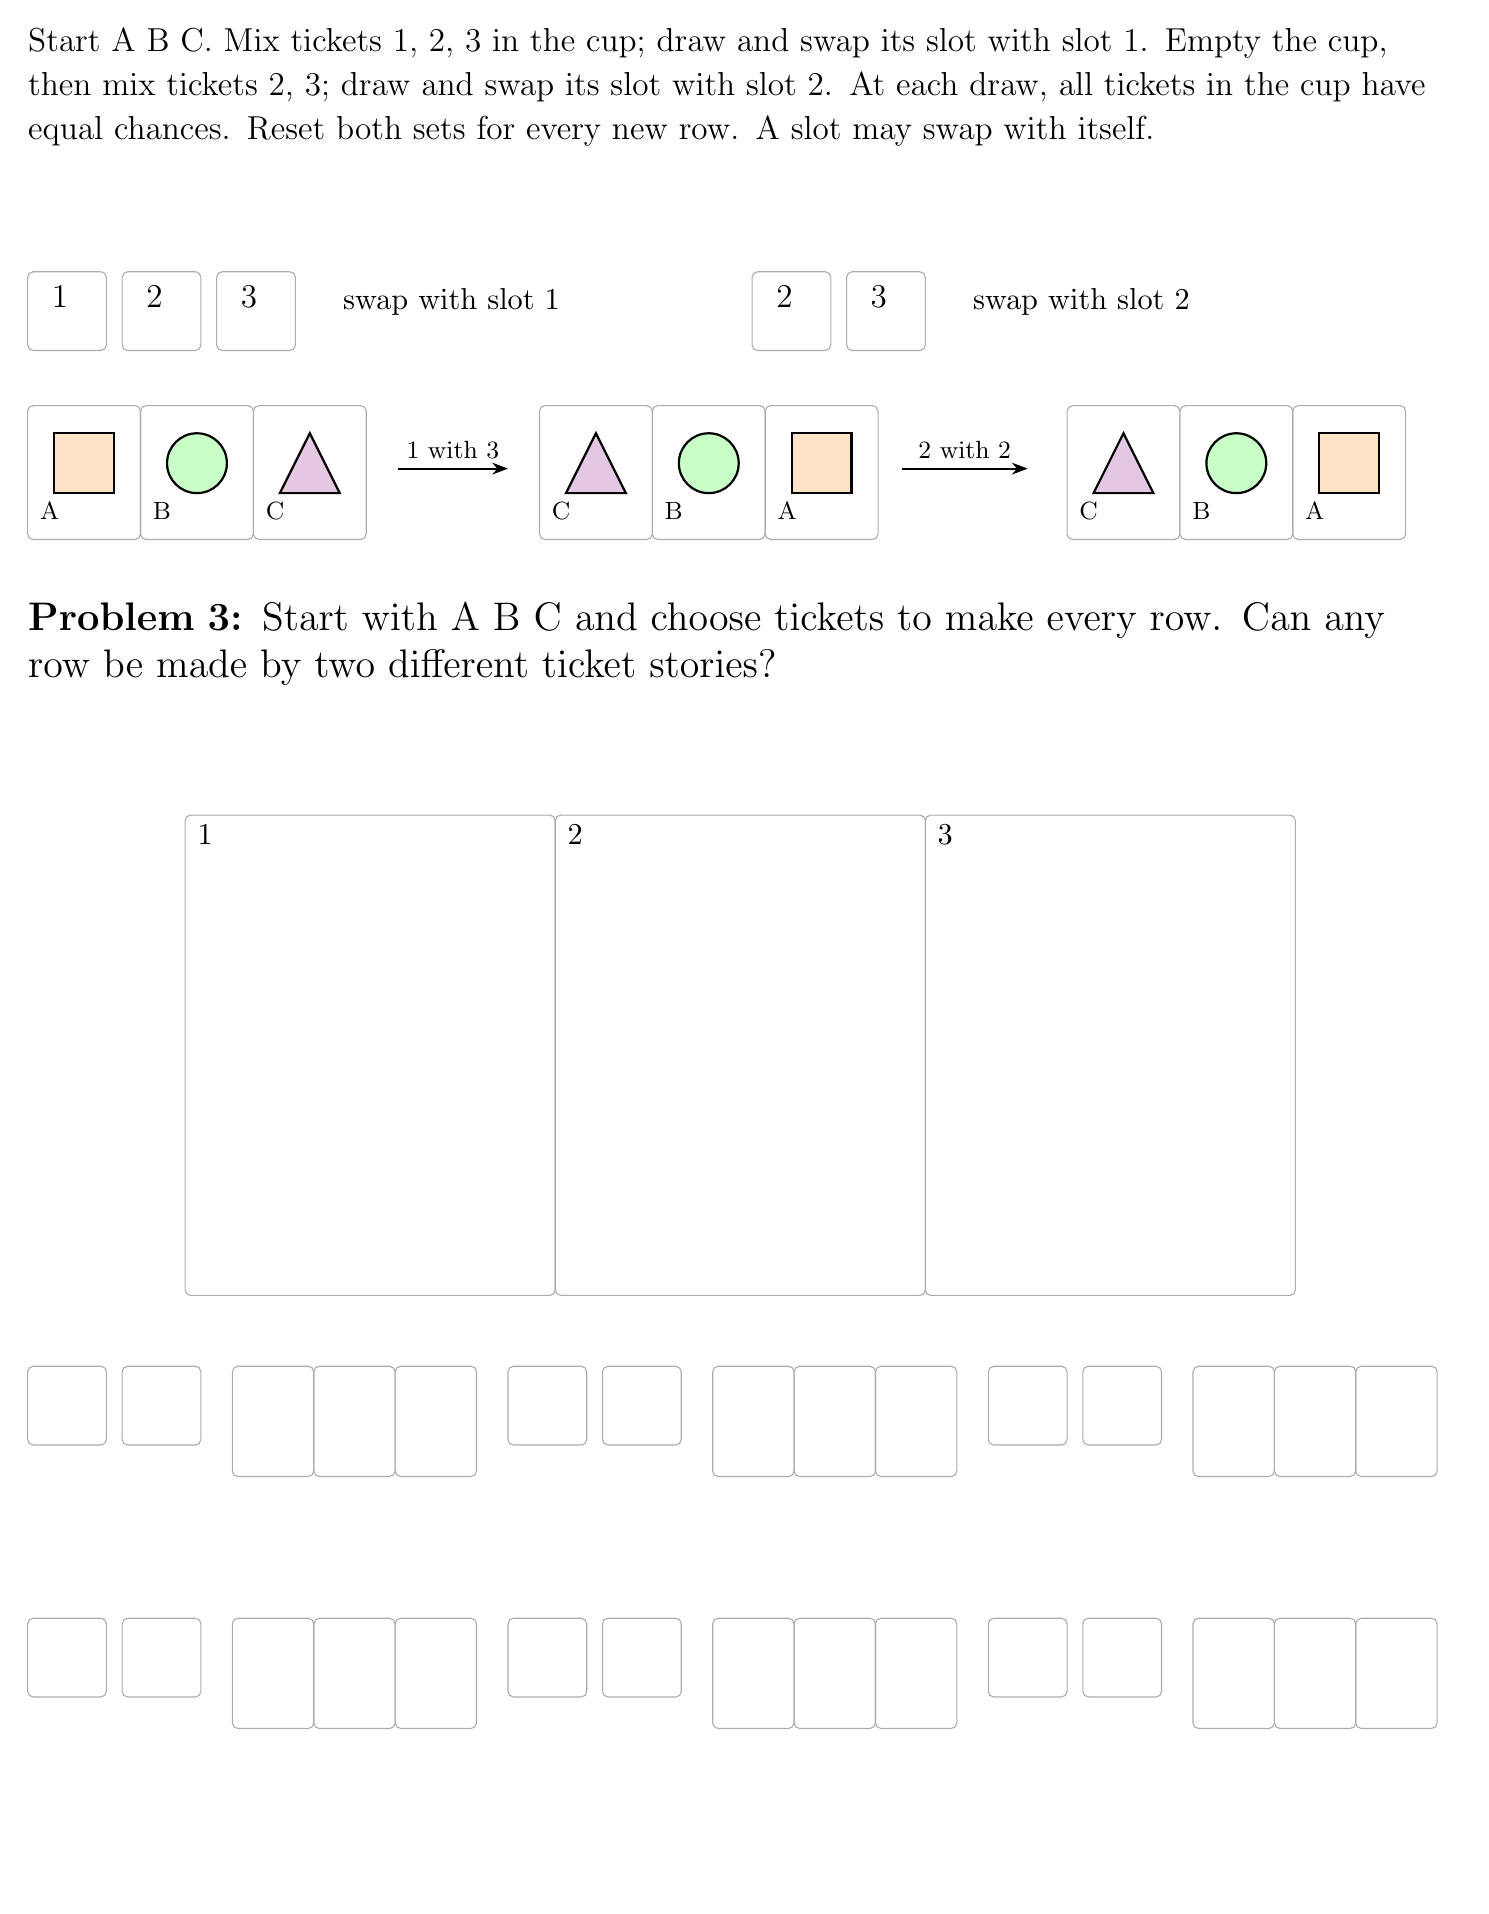
\begin{tikzpicture}[x=1cm,y=1cm]\path[use as bounding box] (0,0) rectangle (18.2,-23.6);
\node[anchor=north west,text width=18cm,inner sep=0pt,font=\fontsize{13}{16}\selectfont] at (0,0) {Start A B C. Mix tickets 1, 2, 3 in the cup; draw and swap its slot with slot 1. Empty the cup, then mix tickets 2, 3; draw and swap its slot with slot 2. At each draw, all tickets in the cup have equal chances. Reset both sets for every new row. A slot may swap with itself.};
\draw[gray!65,rounded corners=2pt] (0.0,-3.1) rectangle (1.0,-4.1);
\node[anchor=north west,text width=0.5cm,inner sep=0pt,font=\fontsize{13}{16}\selectfont] at (0.3,-3.27) {1};
\draw[gray!65,rounded corners=2pt] (1.2,-3.1) rectangle (2.2,-4.1);
\node[anchor=north west,text width=0.5cm,inner sep=0pt,font=\fontsize{13}{16}\selectfont] at (1.5,-3.27) {2};
\draw[gray!65,rounded corners=2pt] (2.4,-3.1) rectangle (3.4,-4.1);
\node[anchor=north west,text width=0.5cm,inner sep=0pt,font=\fontsize{13}{16}\selectfont] at (2.6999999999999997,-3.27) {3};
\node[anchor=north west,text width=5cm,inner sep=0pt,font=\fontsize{11}{14}\selectfont] at (4,-3.3) {swap with slot 1};
\draw[gray!65,rounded corners=2pt] (9.2,-3.1) rectangle (10.2,-4.1);
\node[anchor=north west,text width=0.5cm,inner sep=0pt,font=\fontsize{13}{16}\selectfont] at (9.5,-3.27) {2};
\draw[gray!65,rounded corners=2pt] (10.399999999999999,-3.1) rectangle (11.399999999999999,-4.1);
\node[anchor=north west,text width=0.5cm,inner sep=0pt,font=\fontsize{13}{16}\selectfont] at (10.7,-3.27) {3};
\node[anchor=north west,text width=6cm,inner sep=0pt,font=\fontsize{11}{14}\selectfont] at (12,-3.3) {swap with slot 2};
\draw[gray!65,rounded corners=2pt] (0.0,-4.8) rectangle (1.4333333333333333,-6.5);
\draw[fill=orange!22,line width=.8pt] (0.33666666666666667,-5.911) rectangle (1.0966666666666667,-5.151);
\node[anchor=north west,text width=1.2333333333333334cm,inner sep=0pt,font=\fontsize{9}{12}\selectfont] at (0.15,-6.024) {A};
\draw[gray!65,rounded corners=2pt] (1.4333333333333333,-4.8) rectangle (2.8666666666666667,-6.5);
\draw[fill=green!22,line width=.8pt] (2.15,-5.531) circle (0.38);
\node[anchor=north west,text width=1.2333333333333334cm,inner sep=0pt,font=\fontsize{9}{12}\selectfont] at (1.5833333333333333,-6.024) {B};
\draw[gray!65,rounded corners=2pt] (2.8666666666666667,-4.8) rectangle (4.3,-6.5);
\draw[fill=violet!22,line width=.8pt] (3.5833333333333335,-5.151) -- (3.9633333333333334,-5.911) -- (3.2033333333333336,-5.911) -- cycle;
\node[anchor=north west,text width=1.2333333333333334cm,inner sep=0pt,font=\fontsize{9}{12}\selectfont] at (3.0166666666666666,-6.024) {C};
\draw[-{Stealth[length=2mm]},line width=.8pt] (4.7,-5.6) -- (6.1,-5.6) node[midway,above,font=\small] {1 with 3};
\draw[gray!65,rounded corners=2pt] (6.5,-4.8) rectangle (7.933333333333334,-6.5);
\draw[fill=violet!22,line width=.8pt] (7.216666666666667,-5.151) -- (7.596666666666667,-5.911) -- (6.836666666666667,-5.911) -- cycle;
\node[anchor=north west,text width=1.2333333333333334cm,inner sep=0pt,font=\fontsize{9}{12}\selectfont] at (6.65,-6.024) {C};
\draw[gray!65,rounded corners=2pt] (7.933333333333334,-4.8) rectangle (9.366666666666667,-6.5);
\draw[fill=green!22,line width=.8pt] (8.65,-5.531) circle (0.38);
\node[anchor=north west,text width=1.2333333333333334cm,inner sep=0pt,font=\fontsize{9}{12}\selectfont] at (8.083333333333334,-6.024) {B};
\draw[gray!65,rounded corners=2pt] (9.366666666666667,-4.8) rectangle (10.8,-6.5);
\draw[fill=orange!22,line width=.8pt] (9.703333333333333,-5.911) rectangle (10.463333333333335,-5.151);
\node[anchor=north west,text width=1.2333333333333334cm,inner sep=0pt,font=\fontsize{9}{12}\selectfont] at (9.516666666666667,-6.024) {A};
\draw[-{Stealth[length=2mm]},line width=.8pt] (11.1,-5.6) -- (12.7,-5.6) node[midway,above,font=\small] {2 with 2};
\draw[gray!65,rounded corners=2pt] (13.2,-4.8) rectangle (14.633333333333333,-6.5);
\draw[fill=violet!22,line width=.8pt] (13.916666666666666,-5.151) -- (14.296666666666667,-5.911) -- (13.536666666666665,-5.911) -- cycle;
\node[anchor=north west,text width=1.2333333333333334cm,inner sep=0pt,font=\fontsize{9}{12}\selectfont] at (13.35,-6.024) {C};
\draw[gray!65,rounded corners=2pt] (14.633333333333333,-4.8) rectangle (16.066666666666666,-6.5);
\draw[fill=green!22,line width=.8pt] (15.35,-5.531) circle (0.38);
\node[anchor=north west,text width=1.2333333333333334cm,inner sep=0pt,font=\fontsize{9}{12}\selectfont] at (14.783333333333333,-6.024) {B};
\draw[gray!65,rounded corners=2pt] (16.066666666666666,-4.8) rectangle (17.5,-6.5);
\draw[fill=orange!22,line width=.8pt] (16.403333333333332,-5.911) rectangle (17.16333333333333,-5.151);
\node[anchor=north west,text width=1.2333333333333334cm,inner sep=0pt,font=\fontsize{9}{12}\selectfont] at (16.216666666666665,-6.024) {A};
\node[anchor=north west,text width=18cm,inner sep=0pt,font=\fontsize{14}{17}\selectfont] at (0,-7.3) {\textbf{Problem 3:} Start with A B C and choose tickets to make every row. Can any row be made by two different ticket stories?};
\draw[gray!65,rounded corners=2pt] (2.0,-10) rectangle (6.7,-16.1);
\node[anchor=north west,text width=1cm,inner sep=0pt,font=\fontsize{11}{14}\selectfont] at (2.15,-10.12) {1};
\draw[gray!65,rounded corners=2pt] (6.7,-10) rectangle (11.4,-16.1);
\node[anchor=north west,text width=1cm,inner sep=0pt,font=\fontsize{11}{14}\selectfont] at (6.8500000000000005,-10.12) {2};
\draw[gray!65,rounded corners=2pt] (11.4,-10) rectangle (16.1,-16.1);
\node[anchor=north west,text width=1cm,inner sep=0pt,font=\fontsize{11}{14}\selectfont] at (11.55,-10.12) {3};
\draw[gray!65,rounded corners=2pt] (0.0,-17.0) rectangle (1.0,-18.0);
\node[anchor=north west,text width=0.5cm,inner sep=0pt,font=\fontsize{13}{16}\selectfont] at (0.3,-17.17) {};
\draw[gray!65,rounded corners=2pt] (1.2,-17.0) rectangle (2.2,-18.0);
\node[anchor=north west,text width=0.5cm,inner sep=0pt,font=\fontsize{13}{16}\selectfont] at (1.5,-17.17) {};
\draw[gray!65,rounded corners=2pt] (2.6,-17.0) rectangle (3.6333333333333337,-18.4);
\draw[gray!65,rounded corners=2pt] (3.6333333333333337,-17.0) rectangle (4.666666666666667,-18.4);
\draw[gray!65,rounded corners=2pt] (4.666666666666667,-17.0) rectangle (5.7,-18.4);
\draw[gray!65,rounded corners=2pt] (6.1,-17.0) rectangle (7.1,-18.0);
\node[anchor=north west,text width=0.5cm,inner sep=0pt,font=\fontsize{13}{16}\selectfont] at (6.3999999999999995,-17.17) {};
\draw[gray!65,rounded corners=2pt] (7.3,-17.0) rectangle (8.3,-18.0);
\node[anchor=north west,text width=0.5cm,inner sep=0pt,font=\fontsize{13}{16}\selectfont] at (7.6,-17.17) {};
\draw[gray!65,rounded corners=2pt] (8.7,-17.0) rectangle (9.733333333333333,-18.4);
\draw[gray!65,rounded corners=2pt] (9.733333333333333,-17.0) rectangle (10.766666666666666,-18.4);
\draw[gray!65,rounded corners=2pt] (10.766666666666666,-17.0) rectangle (11.799999999999999,-18.4);
\draw[gray!65,rounded corners=2pt] (12.2,-17.0) rectangle (13.2,-18.0);
\node[anchor=north west,text width=0.5cm,inner sep=0pt,font=\fontsize{13}{16}\selectfont] at (12.5,-17.17) {};
\draw[gray!65,rounded corners=2pt] (13.399999999999999,-17.0) rectangle (14.399999999999999,-18.0);
\node[anchor=north west,text width=0.5cm,inner sep=0pt,font=\fontsize{13}{16}\selectfont] at (13.7,-17.17) {};
\draw[gray!65,rounded corners=2pt] (14.799999999999999,-17.0) rectangle (15.833333333333332,-18.4);
\draw[gray!65,rounded corners=2pt] (15.833333333333332,-17.0) rectangle (16.866666666666667,-18.4);
\draw[gray!65,rounded corners=2pt] (16.866666666666667,-17.0) rectangle (17.900000000000002,-18.4);
\draw[gray!65,rounded corners=2pt] (0.0,-20.2) rectangle (1.0,-21.2);
\node[anchor=north west,text width=0.5cm,inner sep=0pt,font=\fontsize{13}{16}\selectfont] at (0.3,-20.37) {};
\draw[gray!65,rounded corners=2pt] (1.2,-20.2) rectangle (2.2,-21.2);
\node[anchor=north west,text width=0.5cm,inner sep=0pt,font=\fontsize{13}{16}\selectfont] at (1.5,-20.37) {};
\draw[gray!65,rounded corners=2pt] (2.6,-20.2) rectangle (3.6333333333333337,-21.599999999999998);
\draw[gray!65,rounded corners=2pt] (3.6333333333333337,-20.2) rectangle (4.666666666666667,-21.599999999999998);
\draw[gray!65,rounded corners=2pt] (4.666666666666667,-20.2) rectangle (5.7,-21.599999999999998);
\draw[gray!65,rounded corners=2pt] (6.1,-20.2) rectangle (7.1,-21.2);
\node[anchor=north west,text width=0.5cm,inner sep=0pt,font=\fontsize{13}{16}\selectfont] at (6.3999999999999995,-20.37) {};
\draw[gray!65,rounded corners=2pt] (7.3,-20.2) rectangle (8.3,-21.2);
\node[anchor=north west,text width=0.5cm,inner sep=0pt,font=\fontsize{13}{16}\selectfont] at (7.6,-20.37) {};
\draw[gray!65,rounded corners=2pt] (8.7,-20.2) rectangle (9.733333333333333,-21.599999999999998);
\draw[gray!65,rounded corners=2pt] (9.733333333333333,-20.2) rectangle (10.766666666666666,-21.599999999999998);
\draw[gray!65,rounded corners=2pt] (10.766666666666666,-20.2) rectangle (11.799999999999999,-21.599999999999998);
\draw[gray!65,rounded corners=2pt] (12.2,-20.2) rectangle (13.2,-21.2);
\node[anchor=north west,text width=0.5cm,inner sep=0pt,font=\fontsize{13}{16}\selectfont] at (12.5,-20.37) {};
\draw[gray!65,rounded corners=2pt] (13.399999999999999,-20.2) rectangle (14.399999999999999,-21.2);
\node[anchor=north west,text width=0.5cm,inner sep=0pt,font=\fontsize{13}{16}\selectfont] at (13.7,-20.37) {};
\draw[gray!65,rounded corners=2pt] (14.799999999999999,-20.2) rectangle (15.833333333333332,-21.599999999999998);
\draw[gray!65,rounded corners=2pt] (15.833333333333332,-20.2) rectangle (16.866666666666667,-21.599999999999998);
\draw[gray!65,rounded corners=2pt] (16.866666666666667,-20.2) rectangle (17.900000000000002,-21.599999999999998);
\end{tikzpicture}
\newpage
\noindent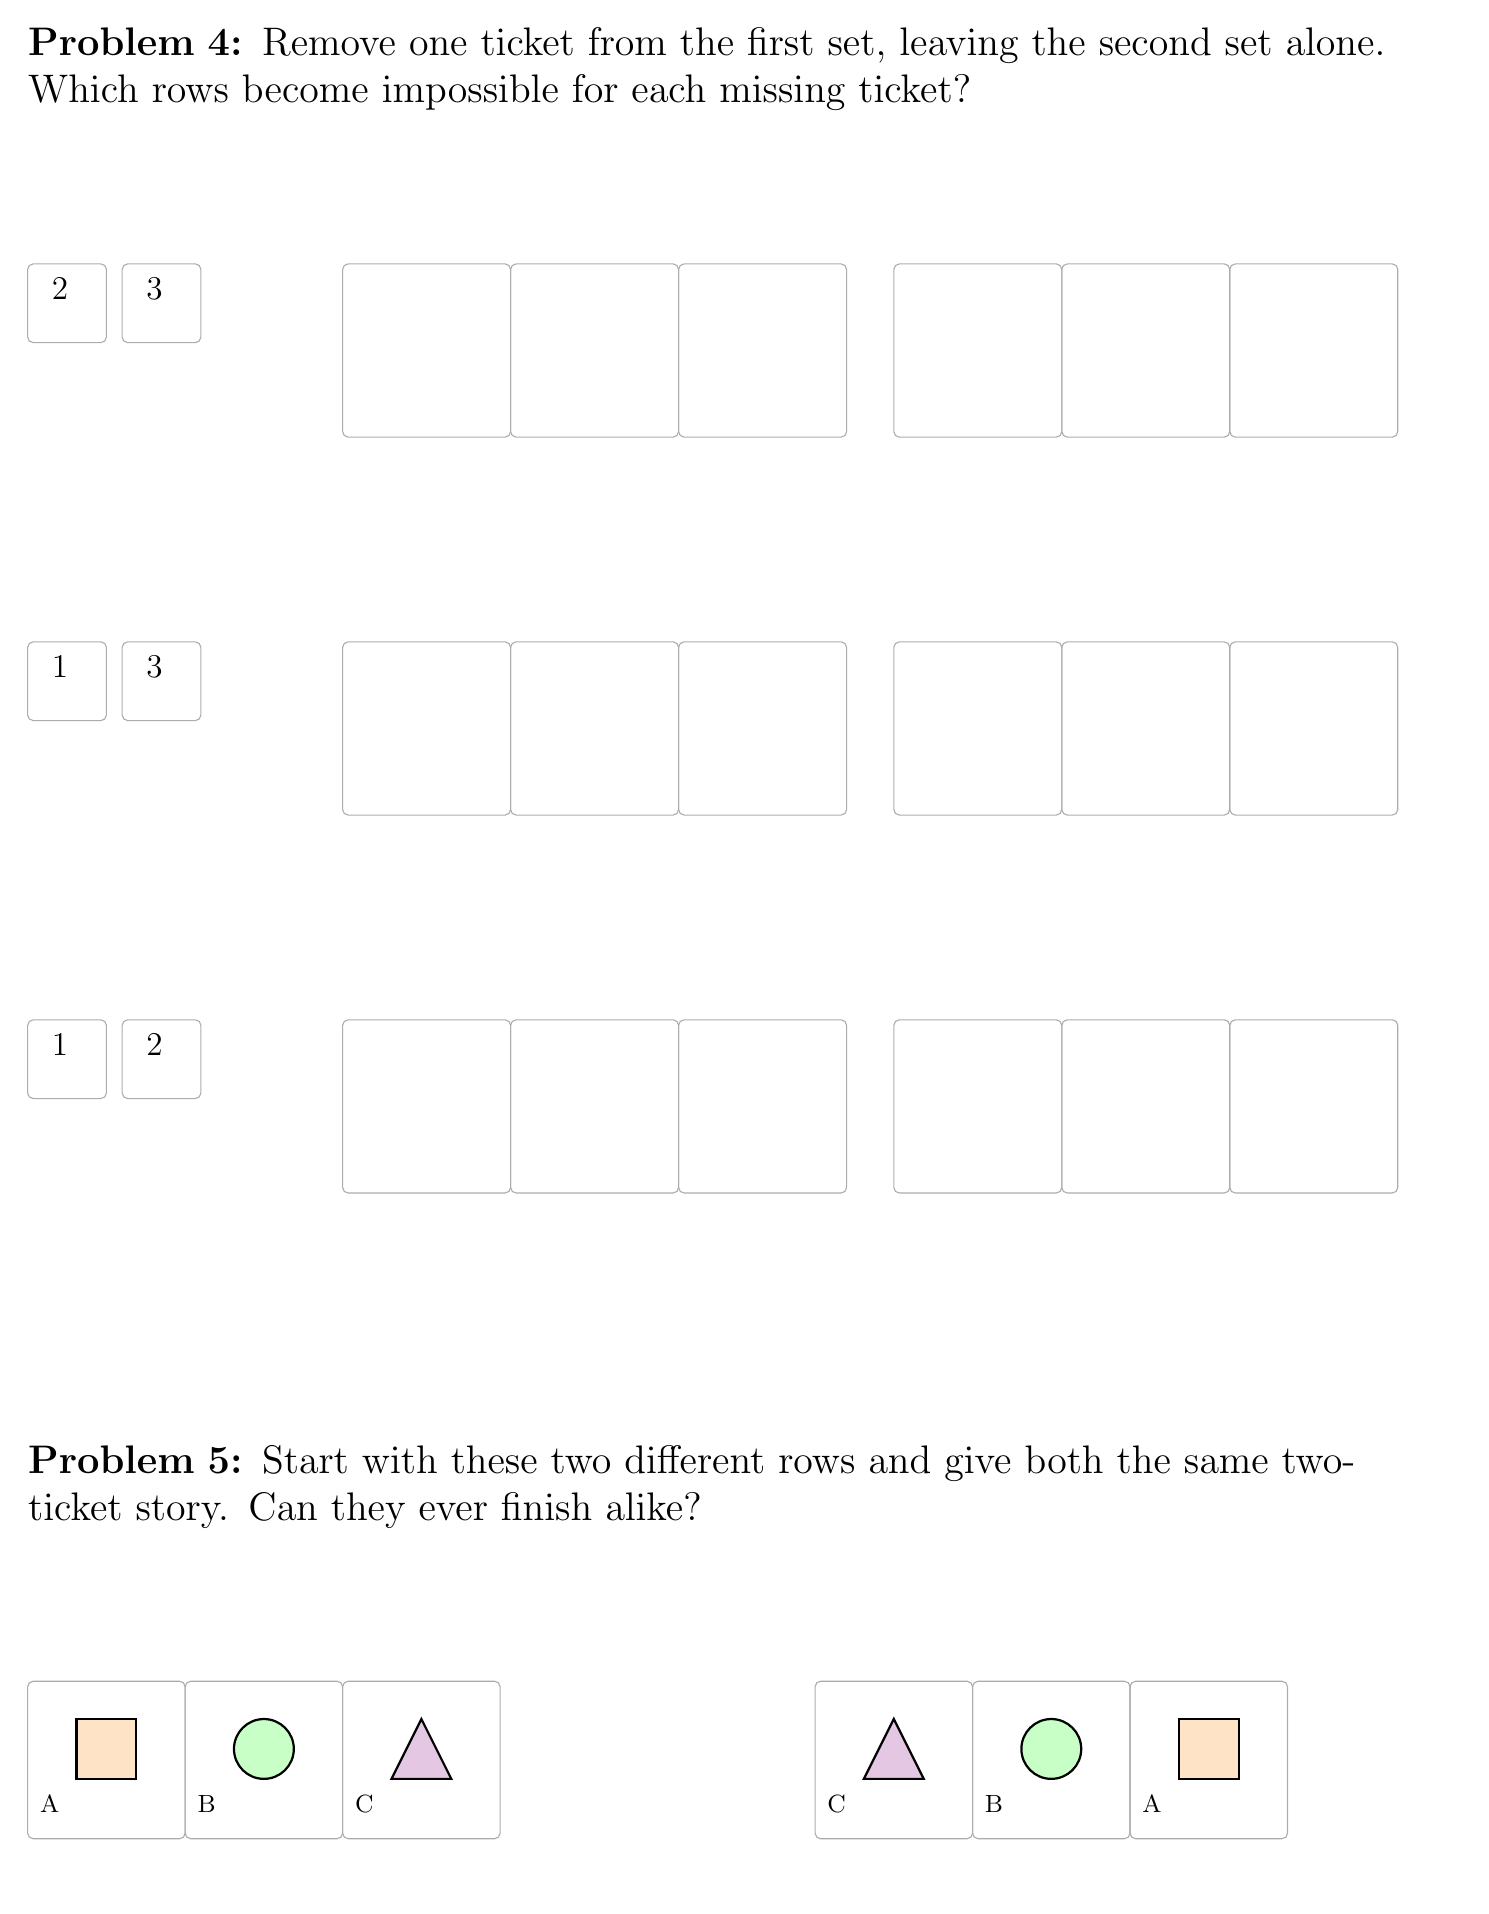
\begin{tikzpicture}[x=1cm,y=1cm]\path[use as bounding box] (0,0) rectangle (18.2,-23.6);
\node[anchor=north west,text width=18cm,inner sep=0pt,font=\fontsize{14}{17}\selectfont] at (0,0) {\textbf{Problem 4:} Remove one ticket from the first set, leaving the second set alone. Which rows become impossible for each missing ticket?};
\draw[gray!65,rounded corners=2pt] (0.0,-3.0) rectangle (1.0,-4.0);
\node[anchor=north west,text width=0.5cm,inner sep=0pt,font=\fontsize{13}{16}\selectfont] at (0.3,-3.17) {2};
\draw[gray!65,rounded corners=2pt] (1.2,-3.0) rectangle (2.2,-4.0);
\node[anchor=north west,text width=0.5cm,inner sep=0pt,font=\fontsize{13}{16}\selectfont] at (1.5,-3.17) {3};
\draw[gray!65,rounded corners=2pt] (4.0,-3.0) rectangle (6.133333333333333,-5.2);
\draw[gray!65,rounded corners=2pt] (6.133333333333333,-3.0) rectangle (8.266666666666666,-5.2);
\draw[gray!65,rounded corners=2pt] (8.266666666666666,-3.0) rectangle (10.399999999999999,-5.2);
\draw[gray!65,rounded corners=2pt] (11.0,-3.0) rectangle (13.133333333333333,-5.2);
\draw[gray!65,rounded corners=2pt] (13.133333333333333,-3.0) rectangle (15.266666666666666,-5.2);
\draw[gray!65,rounded corners=2pt] (15.266666666666666,-3.0) rectangle (17.4,-5.2);
\draw[gray!65,rounded corners=2pt] (0.0,-7.8) rectangle (1.0,-8.8);
\node[anchor=north west,text width=0.5cm,inner sep=0pt,font=\fontsize{13}{16}\selectfont] at (0.3,-7.97) {1};
\draw[gray!65,rounded corners=2pt] (1.2,-7.8) rectangle (2.2,-8.8);
\node[anchor=north west,text width=0.5cm,inner sep=0pt,font=\fontsize{13}{16}\selectfont] at (1.5,-7.97) {3};
\draw[gray!65,rounded corners=2pt] (4.0,-7.8) rectangle (6.133333333333333,-10.0);
\draw[gray!65,rounded corners=2pt] (6.133333333333333,-7.8) rectangle (8.266666666666666,-10.0);
\draw[gray!65,rounded corners=2pt] (8.266666666666666,-7.8) rectangle (10.399999999999999,-10.0);
\draw[gray!65,rounded corners=2pt] (11.0,-7.8) rectangle (13.133333333333333,-10.0);
\draw[gray!65,rounded corners=2pt] (13.133333333333333,-7.8) rectangle (15.266666666666666,-10.0);
\draw[gray!65,rounded corners=2pt] (15.266666666666666,-7.8) rectangle (17.4,-10.0);
\draw[gray!65,rounded corners=2pt] (0.0,-12.6) rectangle (1.0,-13.6);
\node[anchor=north west,text width=0.5cm,inner sep=0pt,font=\fontsize{13}{16}\selectfont] at (0.3,-12.77) {1};
\draw[gray!65,rounded corners=2pt] (1.2,-12.6) rectangle (2.2,-13.6);
\node[anchor=north west,text width=0.5cm,inner sep=0pt,font=\fontsize{13}{16}\selectfont] at (1.5,-12.77) {2};
\draw[gray!65,rounded corners=2pt] (4.0,-12.6) rectangle (6.133333333333333,-14.8);
\draw[gray!65,rounded corners=2pt] (6.133333333333333,-12.6) rectangle (8.266666666666666,-14.8);
\draw[gray!65,rounded corners=2pt] (8.266666666666666,-12.6) rectangle (10.399999999999999,-14.8);
\draw[gray!65,rounded corners=2pt] (11.0,-12.6) rectangle (13.133333333333333,-14.8);
\draw[gray!65,rounded corners=2pt] (13.133333333333333,-12.6) rectangle (15.266666666666666,-14.8);
\draw[gray!65,rounded corners=2pt] (15.266666666666666,-12.6) rectangle (17.4,-14.8);
\node[anchor=north west,text width=18cm,inner sep=0pt,font=\fontsize{14}{17}\selectfont] at (0,-18) {\textbf{Problem 5:} Start with these two different rows and give both the same two-ticket story. Can they ever finish alike?};
\draw[gray!65,rounded corners=2pt] (0.0,-21) rectangle (2.0,-23);
\draw[fill=orange!22,line width=.8pt] (0.62,-22.24) rectangle (1.38,-21.48);
\node[anchor=north west,text width=1.8cm,inner sep=0pt,font=\fontsize{9}{12}\selectfont] at (0.15,-22.44) {A};
\draw[gray!65,rounded corners=2pt] (2.0,-21) rectangle (4.0,-23);
\draw[fill=green!22,line width=.8pt] (3.0,-21.86) circle (0.38);
\node[anchor=north west,text width=1.8cm,inner sep=0pt,font=\fontsize{9}{12}\selectfont] at (2.15,-22.44) {B};
\draw[gray!65,rounded corners=2pt] (4.0,-21) rectangle (6.0,-23);
\draw[fill=violet!22,line width=.8pt] (5.0,-21.48) -- (5.38,-22.24) -- (4.62,-22.24) -- cycle;
\node[anchor=north west,text width=1.8cm,inner sep=0pt,font=\fontsize{9}{12}\selectfont] at (4.15,-22.44) {C};
\draw[gray!65,rounded corners=2pt] (10.0,-21) rectangle (12.0,-23);
\draw[fill=violet!22,line width=.8pt] (11.0,-21.48) -- (11.38,-22.24) -- (10.62,-22.24) -- cycle;
\node[anchor=north west,text width=1.8cm,inner sep=0pt,font=\fontsize{9}{12}\selectfont] at (10.15,-22.44) {C};
\draw[gray!65,rounded corners=2pt] (12.0,-21) rectangle (14.0,-23);
\draw[fill=green!22,line width=.8pt] (13.0,-21.86) circle (0.38);
\node[anchor=north west,text width=1.8cm,inner sep=0pt,font=\fontsize{9}{12}\selectfont] at (12.15,-22.44) {B};
\draw[gray!65,rounded corners=2pt] (14.0,-21) rectangle (16.0,-23);
\draw[fill=orange!22,line width=.8pt] (14.62,-22.24) rectangle (15.38,-21.48);
\node[anchor=north west,text width=1.8cm,inner sep=0pt,font=\fontsize{9}{12}\selectfont] at (14.15,-22.44) {A};
\end{tikzpicture}
\end{document}
